%! TeX program = lualatex
\documentclass[a4paper,11pt]{report}
% packages
\usepackage{censor}
\StopCensoring
\usepackage{fontspec}
\setmainfont{EB Garamond}
% for tironian et fallback
% % \directlua{luaotfload.add_fallback
% % ("emojifallback",
% %      {"Noto Serif:mode=harf"}
% % )}
% % \setmainfont{EB Garamond}[RawFeature={fallback=emojifallback}]

\setmonofont[Scale=MatchLowercase]{Deja Vu Sans Mono}
\usepackage[a4paper,left=2cm,right=2cm,top=\dimexpr15mm+1.5\baselineskip,bottom=2cm]{geometry}
\setlength{\parindent}{0pt}

\usepackage{fancyhdr}       % Headers and footers 
\fancyhead[R]{\normalfont \leftmark}
\fancyhead[L]{}
\pagestyle{fancy}

\usepackage{microtype}      % Slightly tweak font spacing for aesthetics
\usepackage[english]{babel} % Language hyphenation and typographical rules
\usepackage{xcolor}
\definecolor{linkblue}{RGB}{0, 64, 128}
\usepackage[final, colorlinks = false, urlcolor = linkblue]{hyperref} 
% \newcommand{\secref}[1]{\textbf{§~\nameref{#1}}}
\newcommand{\secref}[1]{\textbf{§\ref{#1}~\nameref{#1}}}

\usepackage{changepage}     % adjust margins on the fly

\usepackage[backend=biber, style=numeric, date=iso, urldate=iso]{biblatex}
\addbibresource{references.bib}
\DeclareFieldFormat{urldate}{Accessed on: #1}

\usepackage{minted}
\usemintedstyle{algol_nu}

\usepackage{pgfplots}
\pgfplotsset{width=\textwidth,compat=1.9}

\usepackage{caption}
\newenvironment{code}{\captionsetup{type=listing}}{}
\captionsetup[listing]{skip=0pt}
\setlength{\abovecaptionskip}{5pt}
\setlength{\belowcaptionskip}{5pt}

\usepackage[yyyymmdd]{datetime}
\renewcommand{\dateseparator}{--}

\usepackage{enumitem}

\usepackage{titlesec}

\author{Andrew Hayes}

\begin{document}
\begin{titlepage}
    \begin{center}

        % University Logo
        
\includegraphics[width=0.8\textwidth]{./images/Logo-UGalway-2-3166136658.jpg} \\[1cm]

        % Title
        {\Huge \textbf{Iompar: Live Public Transport Tracking}} \\[0.5cm]
        
        % Department and Degree
        {\Large College of Science \& Engineering} \\[0.3cm]
        {\large Bachelor of Science (Computer Science \& Information Technology)} \\[0.5cm]

        % Report Type
        {\large \textbf{Project Report}} \\[1.5cm]

        % Author Section
        {\Large \textbf{Author:}} \\[0.2cm]
        {\large Andrew Hayes \\ 21321503 } \\[1cm]

        % Supervisor Section
        {\Large \textbf{Academic Supervisor:}} \\[0.2cm]
        {\large Dr. Adrian Clear} \\[1.5cm]

        % Date
        {\Large \today}

    \end{center}
\end{titlepage}

\pagenumbering{roman}
\newpage
\tableofcontents
\newpage
\setcounter{page}{1}
\pagenumbering{arabic}

% yap about mental models with regards to how filters work
% trying to make the application work the same way the user expects it to work

\chapter{Introduction}
\section{Project Overview}
\subsection{Problem Statement}
\subsection{Background}
\section{Document Structure}

\chapter{Research}
\section{Introduction}
\section{Data Sources}
\section{Similar Services}
\section{Technologies}
\subsection{Frontend Technologies}
\subsection{Backend Technologies}
\subsection{Project Management Technologies}
\section{Conclusion}

\chapter{Requirements}
\section{Functional Requirements}
\section{Non-Functional Requirements}
\section{Use Cases}
\section{Constraints}

\chapter{Design}
\section{Backend Design}
\begin{figure}[H]
    \centering
    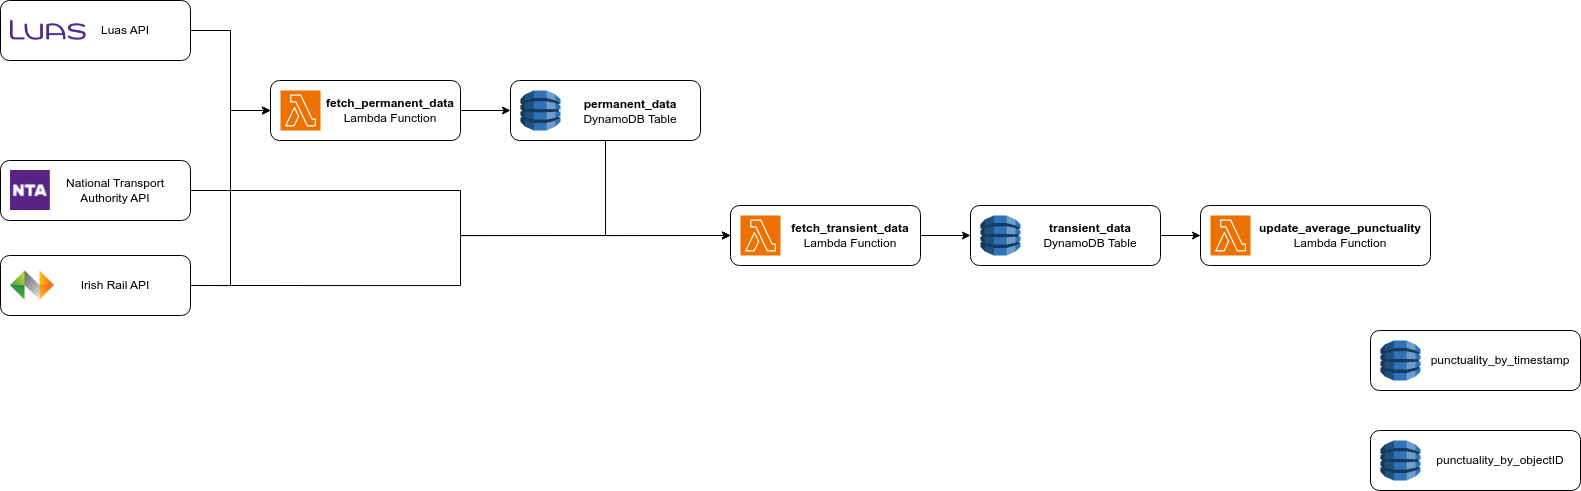
\includegraphics[width=\textwidth]{./images/diagram_all.png}
    \caption{Backend architecture}
\end{figure}

\subsection{Database Design}
Since the chosen database system was DynamoDB, a No-SQL database, the question of how best to separate the data is more open-ended: unlike a relational database, there is no provably correct, optimised structure of separated tables upon which to base the database design.
The decision was made that data would be separated into tables according to the type of data, how its used, and how its updated, thus allowing separation of concerns for functions which update the data and allowing different primary keys and indices to be used for different querying patterns.

\subsubsection{Permanent Data Table}
The permanent data table holds the application data which is unchanging and needs to be updated only rarely, if ever.
This includes information about bus stops, train stations, Luas stops, and bus routes.
The primary key of this table is the \verb|objectID|, necessarily unique to each record in the table.
This is constructed as a combination of the \verb|objectType| (e.g., \verb|BusStop|, \verb|IrishRailStation|) and the unique identifier for that object returned by the API from which the data was retrieved.
The prefix of the \verb|objectType| is used here to guarantee uniqueness of the primary key in the case that two objects in the table of differing types have the same ID given to them by their respective source APIs.
\\\\
There are two ways in which a primary key can be created for a DynamoDB table\supercite{choosing-the-right-key}:
\begin{itemize}
    \item   A simple primary key, consisting solely of a \textbf{partition key}: the attribute which uniquely identifies an item, analogous to simple primary keys in relational database systems.

    \item   A composite primary key, consisting of a partition key and a \textbf{sort key}, analogous to composite primary keys in relational database systems.
            Here, the partition key determines the partition in which an item's data is stored, and the sort key is used to organise the data within that partition.
\end{itemize}

Instead of constructing a new attribute \verb|objectID| for an item, it would also be possible to avoid creating a new attribute by instead using a composite primary key, with the partition key being the item's unique identifier in the system from which it came and the sort key being the \verb|objectType|.
This was rejected in favour of constructing a new attribute, \verb|objectID| to serve as the simple primary key for this table for a number of reasons:
\begin{itemize}
    \item   The uniquely identifying attribute for each item given to it by the API from which said item was sourced has a different attribute name for every API;
            the unique identifier for bus stops is \verb|busStopID|, for train stations is \verb|trainStationCode|, et cetera.
            To use these values as the primary key in the table, each of these attributes would have to be re-named to some single, unifying title, creating additional parsing overhead when the data is being uploaded to the table, and making the item information more difficult to read for humans.

    \item   Having a single uniquely identifying attribute for each item is useful on the frontend, allowing items to be easily uniquely identified without additional processing, useful for user functionality such as adding an item to the user's ``favourites''.

    \item   The query efficiency improvements typically associated with a DynamoDB composite key would not apply to the type of queries this table is designed for with such a composite key structure.
            The data from this table will most often be queried by \verb|objectType| in this application, such as in the event that a user wants to see bus stops or train stations or both on a map.
            The composite key would only speed up querying in the event that, for a number of different items with the same unique identifier, a query was ran on based on the type of those objects sharing an identifier, which is not a situation that is likely to arise for this application.
\end{itemize}

As mentioned in the final bullet-point above, this table is only intended for a single type of query:
queries which seek to return all the items in the table of a certain \verb|objectType| or \verb|objectType|s, such as when a frontend user requests to see bus stops, or train stations, or Luas stops, or some combination of the three.
Therefore, it is imperative that such queries are efficient \& fast. 
Since we cannot partition the data 

\subsection{API Design}
\subsection{Serverless Functions}

\section{Frontend Design}

\chapter{Development}
\section{Introduction}
\section{Backend Development}
\section{Frontend Development}
\section{Development Considerations}

\chapter{Code Quality}
\section{Introduction}
\section{Clean Coding Principles}
\section{Unit Testing}
\section{CI/CD}
\subsection{Continuous Integration}
\subsection{Continuous Deployment}

\chapter{Conclusion}
\section{Evaluation}
\section{Reflection on Requirements}
\section{Reflection on Skill Development}
\section{Potential Future Work}

\printbibliography


\end{document}
